\documentclass[ignorenonframetext,]{beamer}
\setbeamertemplate{caption}[numbered]
\setbeamertemplate{caption label separator}{: }
\setbeamercolor{caption name}{fg=normal text.fg}
\beamertemplatenavigationsymbolsempty
\usepackage{lmodern}
\usepackage{amssymb,amsmath}
\usepackage{ifxetex,ifluatex}
\usepackage{fixltx2e} % provides \textsubscript
\ifnum 0\ifxetex 1\fi\ifluatex 1\fi=0 % if pdftex
  \usepackage[T1]{fontenc}
  \usepackage[utf8]{inputenc}
\else % if luatex or xelatex
  \ifxetex
    \usepackage{mathspec}
  \else
    \usepackage{fontspec}
  \fi
  \defaultfontfeatures{Ligatures=TeX,Scale=MatchLowercase}
\fi
% use upquote if available, for straight quotes in verbatim environments
\IfFileExists{upquote.sty}{\usepackage{upquote}}{}
% use microtype if available
\IfFileExists{microtype.sty}{%
\usepackage{microtype}
\UseMicrotypeSet[protrusion]{basicmath} % disable protrusion for tt fonts
}{}
\newif\ifbibliography
\hypersetup{
            pdftitle={geotopbricks},
            pdfauthor={Emanuele Cordano},
            pdfborder={0 0 0},
            breaklinks=true}
\urlstyle{same}  % don't use monospace font for urls
\usepackage{color}
\usepackage{fancyvrb}
\newcommand{\VerbBar}{|}
\newcommand{\VERB}{\Verb[commandchars=\\\{\}]}
\DefineVerbatimEnvironment{Highlighting}{Verbatim}{commandchars=\\\{\}}
% Add ',fontsize=\small' for more characters per line
\usepackage{framed}
\definecolor{shadecolor}{RGB}{248,248,248}
\newenvironment{Shaded}{\begin{snugshade}}{\end{snugshade}}
\newcommand{\KeywordTok}[1]{\textcolor[rgb]{0.13,0.29,0.53}{\textbf{#1}}}
\newcommand{\DataTypeTok}[1]{\textcolor[rgb]{0.13,0.29,0.53}{#1}}
\newcommand{\DecValTok}[1]{\textcolor[rgb]{0.00,0.00,0.81}{#1}}
\newcommand{\BaseNTok}[1]{\textcolor[rgb]{0.00,0.00,0.81}{#1}}
\newcommand{\FloatTok}[1]{\textcolor[rgb]{0.00,0.00,0.81}{#1}}
\newcommand{\ConstantTok}[1]{\textcolor[rgb]{0.00,0.00,0.00}{#1}}
\newcommand{\CharTok}[1]{\textcolor[rgb]{0.31,0.60,0.02}{#1}}
\newcommand{\SpecialCharTok}[1]{\textcolor[rgb]{0.00,0.00,0.00}{#1}}
\newcommand{\StringTok}[1]{\textcolor[rgb]{0.31,0.60,0.02}{#1}}
\newcommand{\VerbatimStringTok}[1]{\textcolor[rgb]{0.31,0.60,0.02}{#1}}
\newcommand{\SpecialStringTok}[1]{\textcolor[rgb]{0.31,0.60,0.02}{#1}}
\newcommand{\ImportTok}[1]{#1}
\newcommand{\CommentTok}[1]{\textcolor[rgb]{0.56,0.35,0.01}{\textit{#1}}}
\newcommand{\DocumentationTok}[1]{\textcolor[rgb]{0.56,0.35,0.01}{\textbf{\textit{#1}}}}
\newcommand{\AnnotationTok}[1]{\textcolor[rgb]{0.56,0.35,0.01}{\textbf{\textit{#1}}}}
\newcommand{\CommentVarTok}[1]{\textcolor[rgb]{0.56,0.35,0.01}{\textbf{\textit{#1}}}}
\newcommand{\OtherTok}[1]{\textcolor[rgb]{0.56,0.35,0.01}{#1}}
\newcommand{\FunctionTok}[1]{\textcolor[rgb]{0.00,0.00,0.00}{#1}}
\newcommand{\VariableTok}[1]{\textcolor[rgb]{0.00,0.00,0.00}{#1}}
\newcommand{\ControlFlowTok}[1]{\textcolor[rgb]{0.13,0.29,0.53}{\textbf{#1}}}
\newcommand{\OperatorTok}[1]{\textcolor[rgb]{0.81,0.36,0.00}{\textbf{#1}}}
\newcommand{\BuiltInTok}[1]{#1}
\newcommand{\ExtensionTok}[1]{#1}
\newcommand{\PreprocessorTok}[1]{\textcolor[rgb]{0.56,0.35,0.01}{\textit{#1}}}
\newcommand{\AttributeTok}[1]{\textcolor[rgb]{0.77,0.63,0.00}{#1}}
\newcommand{\RegionMarkerTok}[1]{#1}
\newcommand{\InformationTok}[1]{\textcolor[rgb]{0.56,0.35,0.01}{\textbf{\textit{#1}}}}
\newcommand{\WarningTok}[1]{\textcolor[rgb]{0.56,0.35,0.01}{\textbf{\textit{#1}}}}
\newcommand{\AlertTok}[1]{\textcolor[rgb]{0.94,0.16,0.16}{#1}}
\newcommand{\ErrorTok}[1]{\textcolor[rgb]{0.64,0.00,0.00}{\textbf{#1}}}
\newcommand{\NormalTok}[1]{#1}
\usepackage{graphicx,grffile}
\makeatletter
\def\maxwidth{\ifdim\Gin@nat@width>\linewidth\linewidth\else\Gin@nat@width\fi}
\def\maxheight{\ifdim\Gin@nat@height>\textheight0.8\textheight\else\Gin@nat@height\fi}
\makeatother
% Scale images if necessary, so that they will not overflow the page
% margins by default, and it is still possible to overwrite the defaults
% using explicit options in \includegraphics[width, height, ...]{}
\setkeys{Gin}{width=\maxwidth,height=\maxheight,keepaspectratio}

% Prevent slide breaks in the middle of a paragraph:
\widowpenalties 1 10000
\raggedbottom

\AtBeginPart{
  \let\insertpartnumber\relax
  \let\partname\relax
  \frame{\partpage}
}
\AtBeginSection{
  \ifbibliography
  \else
    \let\insertsectionnumber\relax
    \let\sectionname\relax
    \frame{\sectionpage}
  \fi
}
\AtBeginSubsection{
  \let\insertsubsectionnumber\relax
  \let\subsectionname\relax
  \frame{\subsectionpage}
}

\setlength{\parindent}{0pt}
\setlength{\parskip}{6pt plus 2pt minus 1pt}
\setlength{\emergencystretch}{3em}  % prevent overfull lines
\providecommand{\tightlist}{%
  \setlength{\itemsep}{0pt}\setlength{\parskip}{0pt}}
\setcounter{secnumdepth}{0}
%% EMOS rmarkdown/beamer header
%% Mark van der Loo (2016)
\usepackage{listings}
\usepackage{mdframed}
\usepackage{tikz}

\usetikzlibrary{arrows, positioning, decorations.pathreplacing} 
\usepackage{pgfplots}
\usepackage{color}


% CBS corporate light blue
\definecolor{corplightblue}{HTML}{00a1cd}
% CBS corporate dark blue
\definecolor{corpdarkblue}{HTML}{0058b8}

% set title colors
\setbeamercolor{frametitle}{fg=corpdarkblue}
\setbeamercolor{title}{fg=corpdarkblue}
\setbeamercolor{block title}{fg=corpdarkblue}

\setbeamerfont{normal text}{parent=structure}
% nicer, rounder font for title
\setbeamerfont{title}{series=\bfseries,parent=structure}
% frame titles in boldface
\setbeamerfont{frametitle}{series=\bfseries}
% block title font
\setbeamerfont{block title}{parent=structure}

% enumeration
\setbeamertemplate{itemize item}{\color{corpdarkblue}$\blacktriangleright$}
\setbeamertemplate{itemize subitem}{\color{corpdarkblue}$-$}
\setbeamercolor*{enumerate item}{fg=corpdarkblue}
\setbeamercolor*{enumerate subitem}{fg=corpdarkblue}
\setbeamercolor*{enumerate subsubitem}{fg=corpdarkblue}


\makeatletter
\newcommand\HUGE{\@setfontsize\Huge{50}{60}}
\makeatother    


% nicer, rounder font for title

\setbeamertemplate{title page}{
\begin{picture}(0,0)
\put(0,50){\usebeamerfont{title}{\textcolor{corpdarkblue}{\inserttitle}\par}}

\put(0,20){
\small Emanuele Cordano, Rendena100
}
\put(0,0){
\texttt{\small @ecor} | \texttt{\small github.com/ecor}
}


\put(150,-100){

\includegraphics[height=3cm]{resources/logo/logo_useR2019.png}
}
\end{picture}

}



\setbeamertemplate{frametitle}
{
  \begin{beamercolorbox}{frametitle}
  \vskip2.7ex\insertframetitle
  \end{beamercolorbox}
}


% remove the space-eating navigation symbols
\beamertemplatenavigationsymbolsempty

% convenience function to define rgb colors in tikz
\tikzset{xcolor/.code args={#1=#2}{
     \definecolor{mytemp}{rgb}{#2}
     \tikzset{#1=mytemp}
  }
}


\usebackgroundtemplate{
   \begin{picture}(0,0)
    \put(270, -273){%
      \raisebox{5mm}{\tiny useR2019, Toulouse,France }
\includegraphics[height=8mm]{resources/logo/logo_useR2019.png}
    }
\put(0,-273){

\includegraphics[height=7mm]{resources/logo/logo_geotop.jpeg}

\includegraphics[height=7mm]{resources/logo/logo_eurac.png}

\includegraphics[height=7mm]{resources/logo/logo_rendena100_textoutside_small.jpg}
}
\end{picture}
}


\newcommand{\la}[1]{\boldsymbol{#1}}


\def\begincols{\begin{columns}}
\def\begincol{\begin{column}}
\def\endcol{\end{column}}
\def\endcols{\end{columns}}

\title{geotopbricks}
\subtitle{An R Package for the Distributed Hydrological Model GEOtop}
\author{Emanuele Cordano}
\date{github/ecor / useR2019}

\begin{document}
\frame{\titlepage}

\begin{frame}[fragile]{Who are we?}

\begin{itemize}
\tightlist
\item
  Environmental engineer with hydraulic and hydrological background
  (more deterministic and physicall-based than statics!)
\item
  Some skills in programming and a R entusiast which I use to work with
  hydro-climatic data.
\item
  Find me as @ecor on GitHub
\item
  I'm self-employed and freelancer as www.rendena100.eu .\\
\item
  Author of several R-packages and p
\item
  the other authors?
\item
  Hydrologist ,,, BLA elisa, Giaomo
\item
  Author of several packages, including \texttt{geotop},\ldots{}
\item
  inserire immagini degli autori
\end{itemize}

\end{frame}

\begin{frame}{Hydrology}

Scientific study of the movement, distribution, and quality of water on
Earth water cycle, water resources and environmental watershed
sustainability (REF)

\begin{figure}
\centering
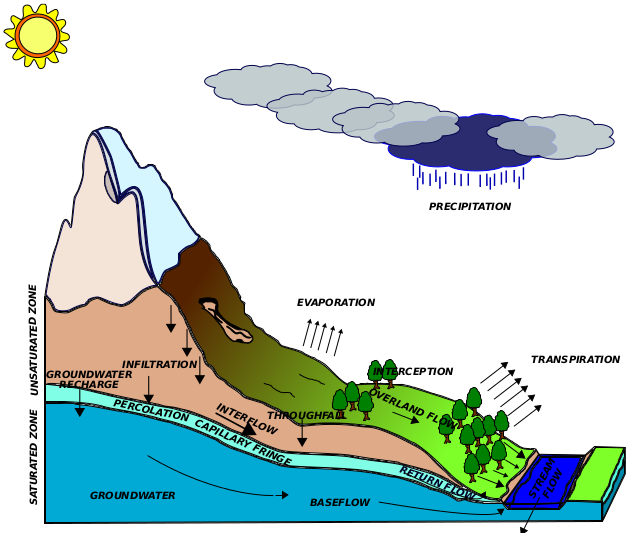
\includegraphics[width=0.50000\textwidth]{resources/images/geotop_landscape.png}
\caption{}
\end{figure}

\end{frame}

\begin{frame}{Hydrolgical models}

\begincols
 \begincol{.48\textwidth}

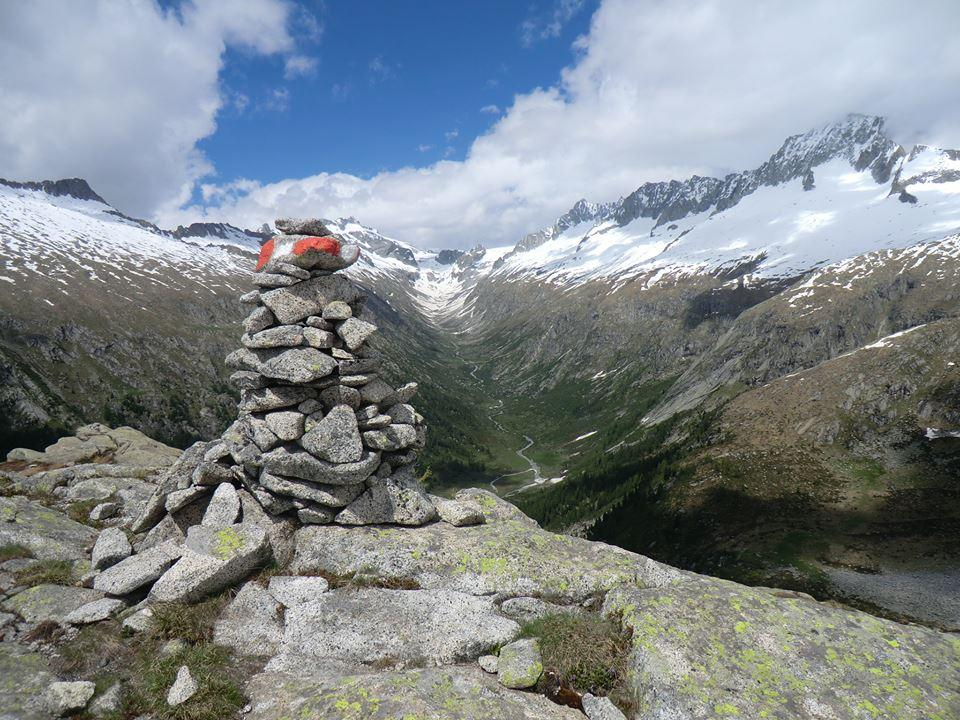
\includegraphics[width=1.00000\textwidth]{resources/images/valdifumo.jpg}~

\endcol
\begincol{.48\textwidth} \begincols
 \begincol{.48\textwidth}
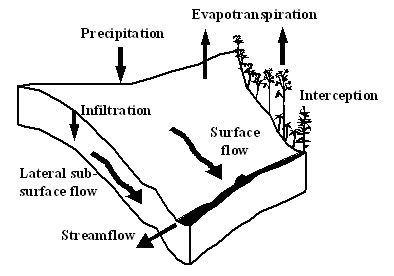
\includegraphics[width=1.00000\textwidth]{resources/images/versante1.png}\\

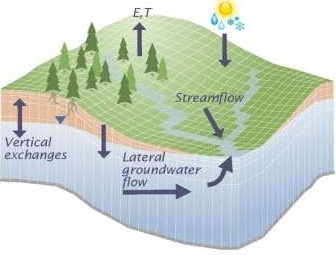
\includegraphics[width=1.00000\textwidth]{resources/images/integrated_models.jpg}\\
\endcol
\begincol{.48\textwidth}
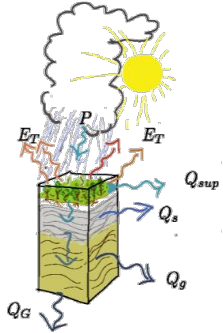
\includegraphics[width=1.00000\textwidth]{resources/images/water_balance.png}\\
\endcol
 \endcols
 \endcol
\endcols

\end{frame}

\begin{frame}{GEOtop Hydrological Model}

GEOtop is an open-source integrated hydrological model that simulates:

\begin{itemize}
\item water flow in the soil $\,\to\,$ Richards' eq (sub) + Kinematic eq (sur)
\item energy exchange with the atmosphere $\,\to\,$ full integration of equation
\end{itemize}

Metti alcune referenze + link github

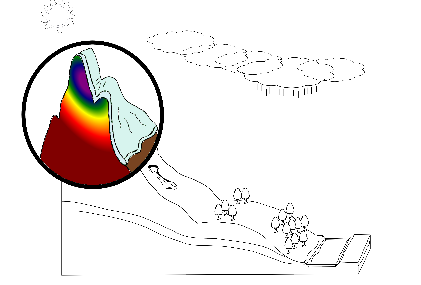
\includegraphics[width=0.20000\textwidth]{resources/images/geotop_snow.png}\\
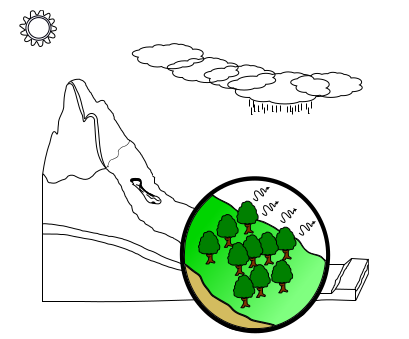
\includegraphics[width=0.20000\textwidth]{resources/images/geotop_vegetation.png}\\
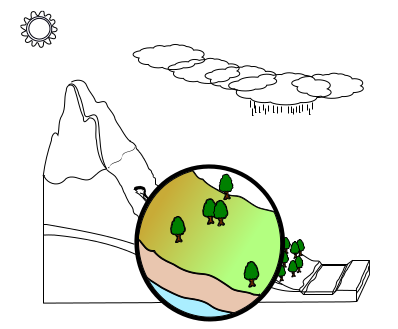
\includegraphics[width=0.20000\textwidth]{resources/images/geotop_infiltration.png}\\

\end{frame}

\begin{frame}{Hydrological Model Structure}

\begin{itemize}
\tightlist
\item
  Input: meteo data, elevations, soil parameters
\item
  Output: snow cover, soil temperature, soil moisture
\item
  \textbf{Semplifica il grafico con solo input e output e processi
  principali}
\end{itemize}

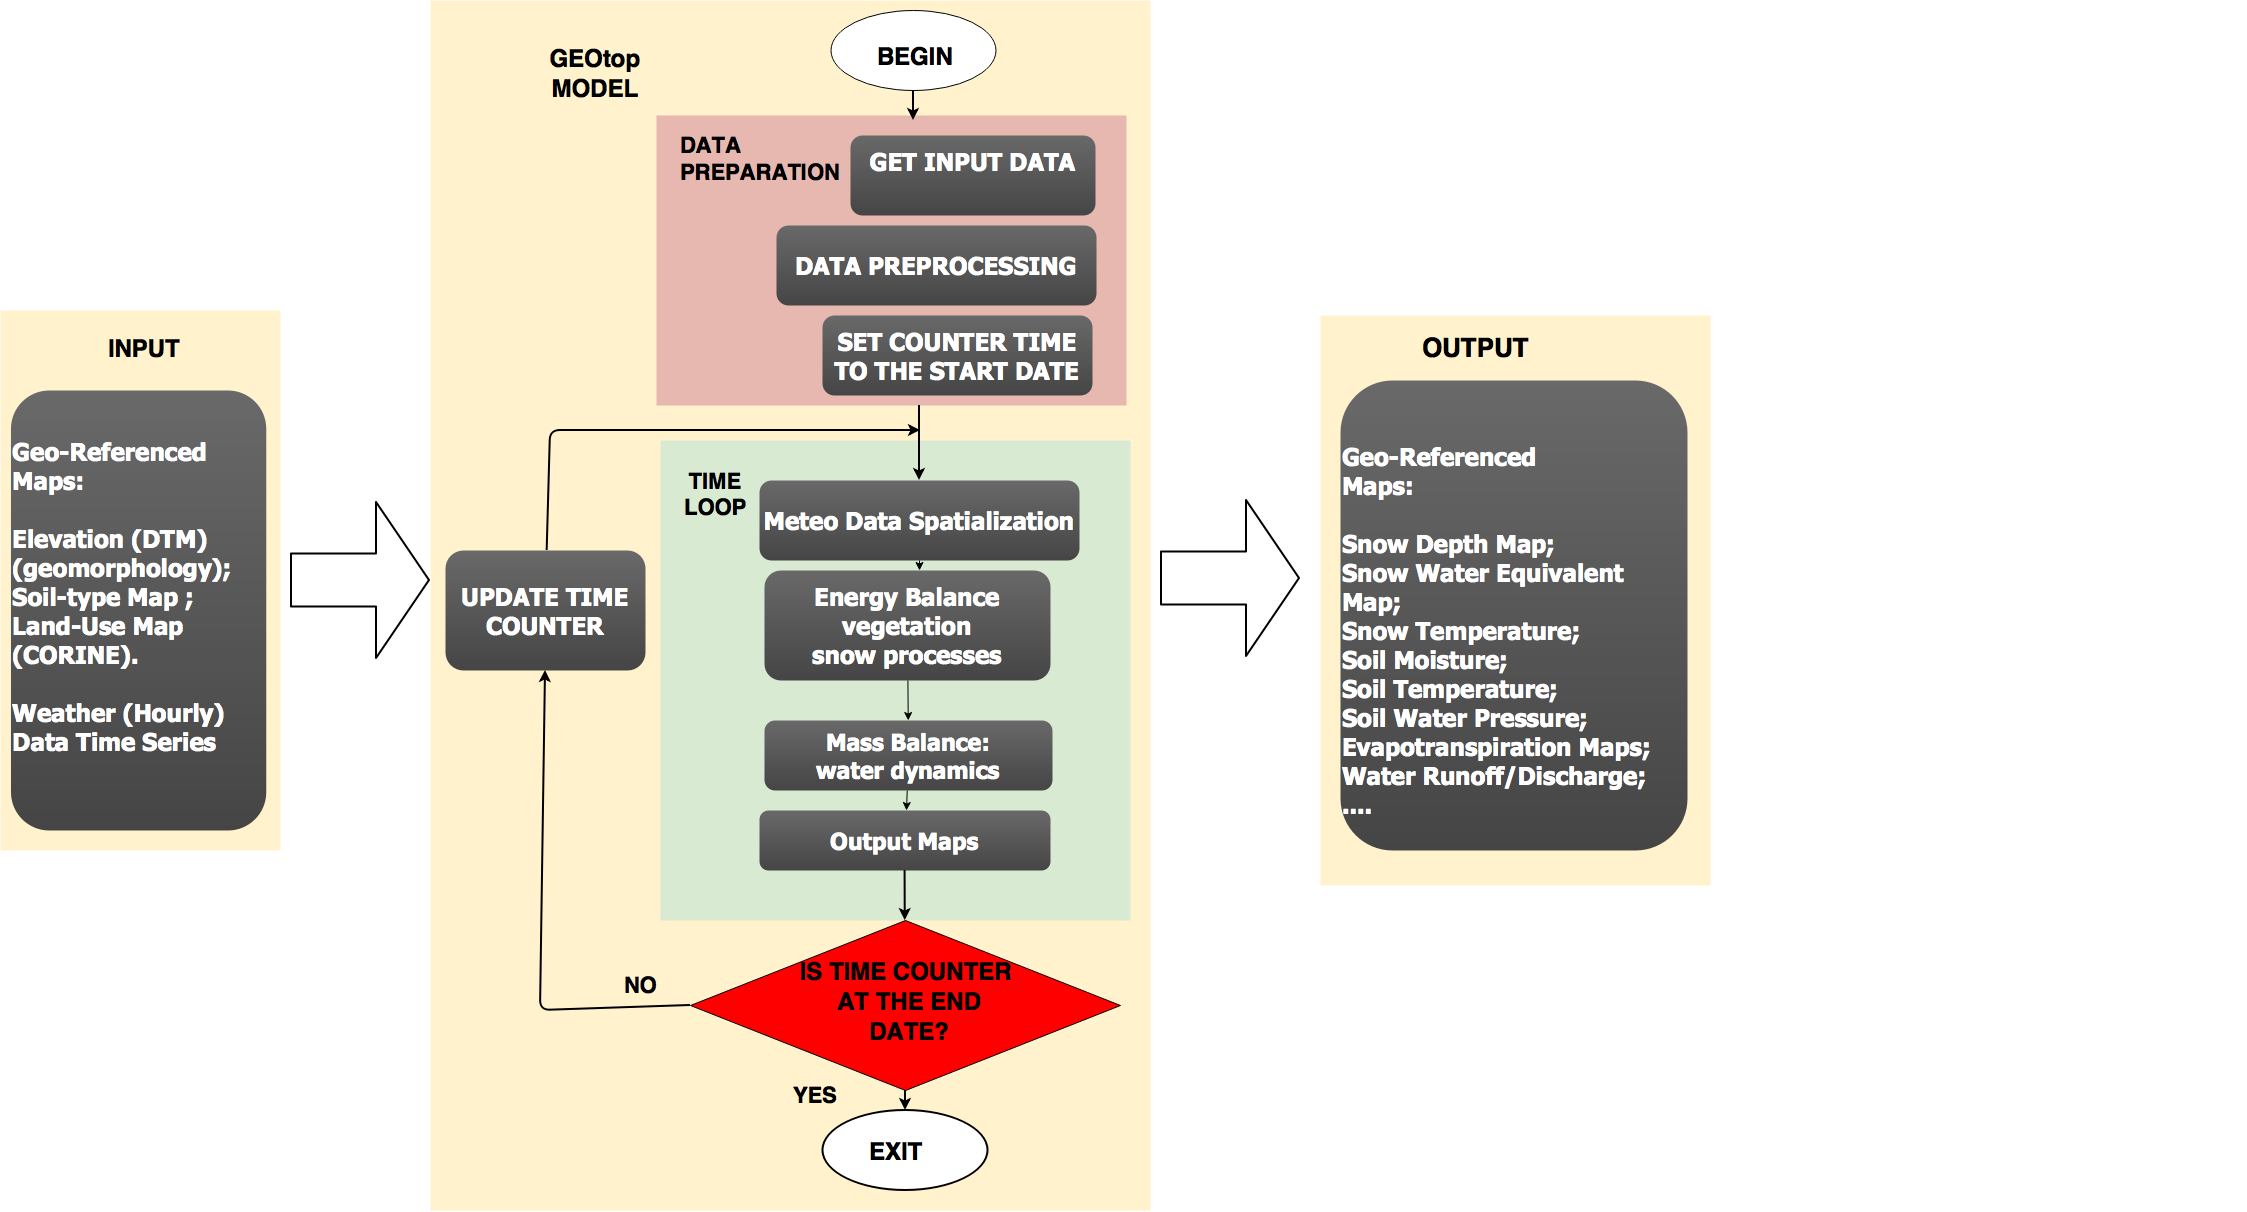
\includegraphics[width=0.90000\textwidth]{resources/images/geotop_revised.png}\\

\end{frame}

\begin{frame}{GEOtop model Optional Subtitle}

Water and energy budgets can be activated :

\begin{itemize}
\tightlist
\item
  one or the other \(\,\to\,\) simplification
\item
  both them together \(\,\to\,\) realistic
\end{itemize}

Two setup configurations : - \textbf{1D}: only vertical fluxes
\(\,\to\,\) mass and energy balance at local scale (only in one soil
column) - \textbf{3D}: vertical and lateral fluxes \(\,\to\,\) balances
at basin scale

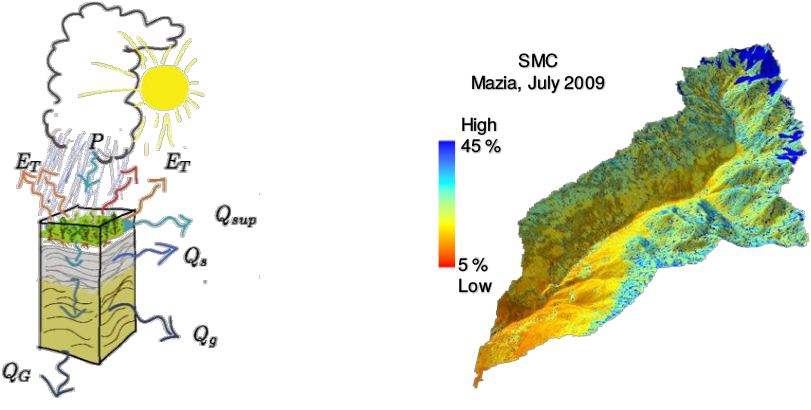
\includegraphics[width=0.90000\textwidth]{resources/images/geotop_ET_SWC.png}\\
\#\# GEOtop model Optional Subtitle

Core components of GEOtop software packages are:

\begin{itemize}
\tightlist
\item
  written in C/C++
\item
  released in 2014 (version 2.0) as free open-source project, a
  re-engineering process is going to finish (version 3.0);
\item
  scientifically tested and published;
\item
  documented on GitHub repository:
  *\url{http://geotopmodel.github.io/geotop/*}
\end{itemize}


\includegraphics[width=0.90000\textwidth]{resources/images/geotop_paper_2017.png}\\

\end{frame}

\begin{frame}{Motivations}

\begin{itemize}
\tightlist
\item
  complexity in input/output/configuration files and data difficult to
  manage
\end{itemize}

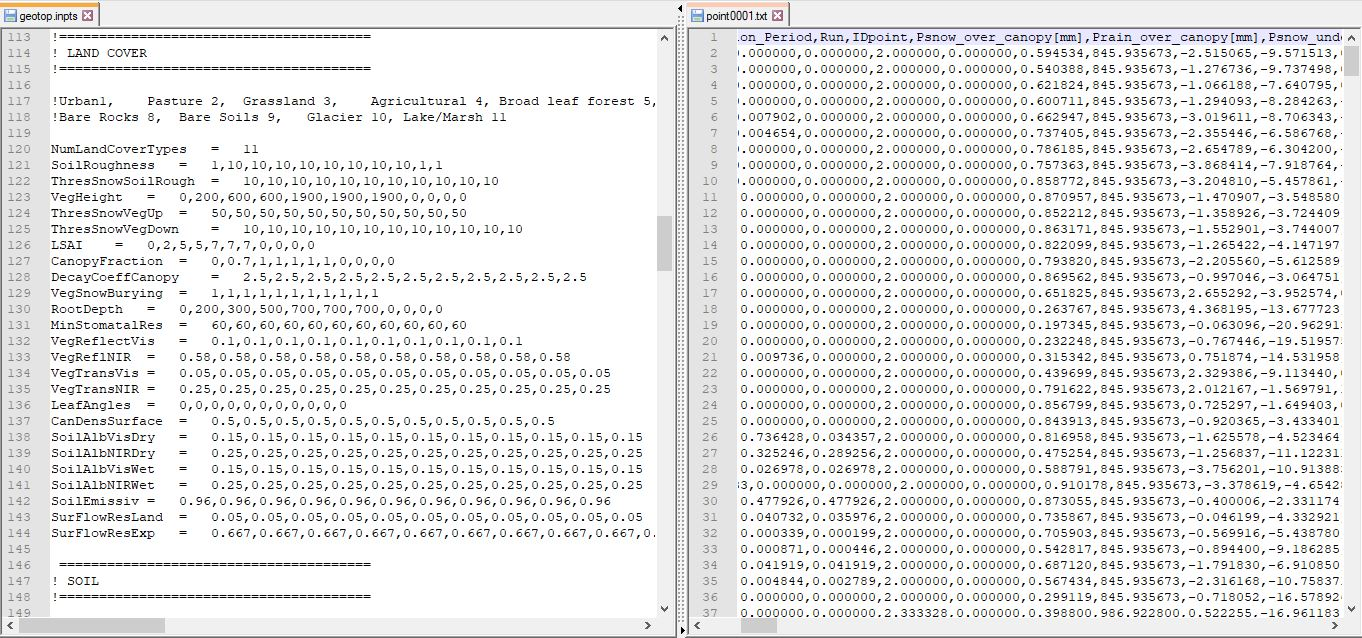
\includegraphics[width=0.90000\textwidth]{resources/images/Capture_IO_GEOtopJPG.JPG}\\
- need of user friendly environment for to GEOtop data tidying and data
analytics (e.g. \emph{R}) - potential interactions between hydrology
(GEOtop) and other knowledge domains (\emph{discipines}).

\end{frame}

\begin{frame}[fragile]{GEOtop configuration File (geotop.inpts)}

A GEOtop simulation is organized in a set of files within a directory
containing a \textbf{configuration file} ,called \emph{geotop.inpts}
filled with a keywords system addressing to:

\begincols
 \begincol{.30\textwidth}

\begin{itemize}
\tightlist
\item
  simulation options (e.g.~simulation period)
\item
  \textbf{input files} (e.g.~meterological time series)
\item
  \textbf{output files}
\end{itemize}

\endcol
 \begincol{.65\textwidth}

\begin{verbatim}
InitDateDDMMYYYYhhmm=09/04/2014 18:00  
EndDateDDMMYYYYhhmm =01/01/2016 00:00 
[...] 
MeteoFile           ="meteoB2_irr" 
PointOutputFile     ="tabs/point" 
\end{verbatim}

\endcol
\endcols

\end{frame}

\begin{frame}[fragile]{\textbf{geotopbricks}}

The aim of \textbf{geotopbricks} , starting in 2013, is to bring all the
data of a GEOtop simulaton into the powerful statistical \textbf{R}
environment by using the \texttt{keyword-value} syntax of
\emph{geotop.inpts}. \textbf{geotopbricks} does the following actions:

\begin{itemize}
\tightlist
\item
  to parse \emph{geotop.inpts} configuration files;
\item
  to derive from \emph{geotop.inpts}'s keywords the source files of I/O
  data;
\item
  to import time series (e.g.~precipitation, temperature, soil water
  content, snow) as \emph{zoo} or \emph{data.frame} objects;
\item
  to import spatially and spatio-temporal gridded objects as
  \emph{RasterLayer-class} or \emph{RasterBrick-class} objects
  (\textbf{raster} package)
\end{itemize}

\end{frame}

\begin{frame}{\textbf{geotopcks} Application 1: Simulation of soil water
budget in an alpine site}

Here is an example on how to extract soil water content (SWC) at a 18cm
depth in two sites P2 and B2, located in Val Mazia/Match, Malles
Venosta/Mals Vinschgau, in South Tyrol, Italy (LOng Term Reasearch
Ecological Area, {[}\url{http://lter.eurac.edu/en}{]}). The goal of the
code lines below is to represent the distribution of soil water content
in August per different years (e.g.~from 2010 to 2014)\\
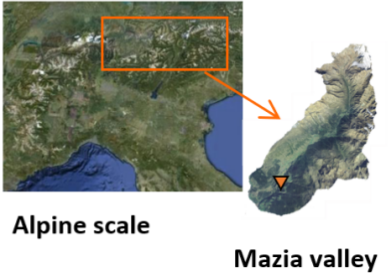
\includegraphics[width=0.40000\textwidth]{resources/images/mazia_2.png}\\

\end{frame}

\begin{frame}[fragile]{Simulation of soil water budget in an alpine
site}

Here is the directory containing files of B2 point simulation:

\begin{Shaded}
\begin{Highlighting}[]
\KeywordTok{library}\NormalTok{(geotopbricks) }

\NormalTok{## SET GEOTOP WORKING DIRECTORY}
\NormalTok{wpath_B2 <-}\StringTok{ "resources/simulation/Matsch_B2_Ref_007"} 
\NormalTok{##writeLines(list.files(wpath_B2))}
\end{Highlighting}
\end{Shaded}

\end{frame}

\begin{frame}[fragile]{Getting simulation input data}

Meteorological variable time series are imported and saved as `meteo'
variable (class `zoo'). This variable is retrieved through the GEOtop
keyword \textbf{MeteoFile} :

\begin{Shaded}
\begin{Highlighting}[]
\NormalTok{tz <-}\StringTok{ "Etc/GMT-1"}
\NormalTok{meteo <-}\StringTok{ }\KeywordTok{get.geotop.inpts.keyword.value}\NormalTok{(}
  \StringTok{"MeteoFile"}\NormalTok{,}
  \DataTypeTok{wpath=}\NormalTok{wpath_B2,}
  \DataTypeTok{data.frame=}\OtherTok{TRUE}\NormalTok{,}
  \DataTypeTok{tz=}\NormalTok{tz)}
\KeywordTok{class}\NormalTok{(meteo)}
\end{Highlighting}
\end{Shaded}

\begin{verbatim}
## [1] "zoo"
\end{verbatim}

\end{frame}

\begin{frame}[fragile]{Getting simulation input data (verify)}

Meteorological time series once imported are available in the R
environment:

\begin{Shaded}
\begin{Highlighting}[]
\KeywordTok{head}\NormalTok{(meteo[}\DecValTok{12}\OperatorTok{:}\DecValTok{14}\NormalTok{,}\KeywordTok{c}\NormalTok{(}\StringTok{"Iprec"}\NormalTok{,}\StringTok{"AirT"}\NormalTok{,}\StringTok{"Swglobal"}\NormalTok{)])}
\end{Highlighting}
\end{Shaded}

\begin{verbatim}
##                     Iprec  AirT Swglobal
## 2009-10-02 11:00:00     0 12.38   396.02
## 2009-10-02 12:00:00     0 13.12   500.07
## 2009-10-02 13:00:00     0 13.96   564.02
\end{verbatim}

\begin{Shaded}
\begin{Highlighting}[]
\KeywordTok{head}\NormalTok{(meteo[}\DecValTok{12}\OperatorTok{:}\DecValTok{14}\NormalTok{,}\KeywordTok{c}\NormalTok{(}\StringTok{"RelHum"}\NormalTok{,}\StringTok{"WindSp"}\NormalTok{,}\StringTok{"WindDir"}\NormalTok{)])}
\end{Highlighting}
\end{Shaded}

\end{frame}

\begin{frame}{Plots of weather variables in B2}

\begin{figure}
\centering
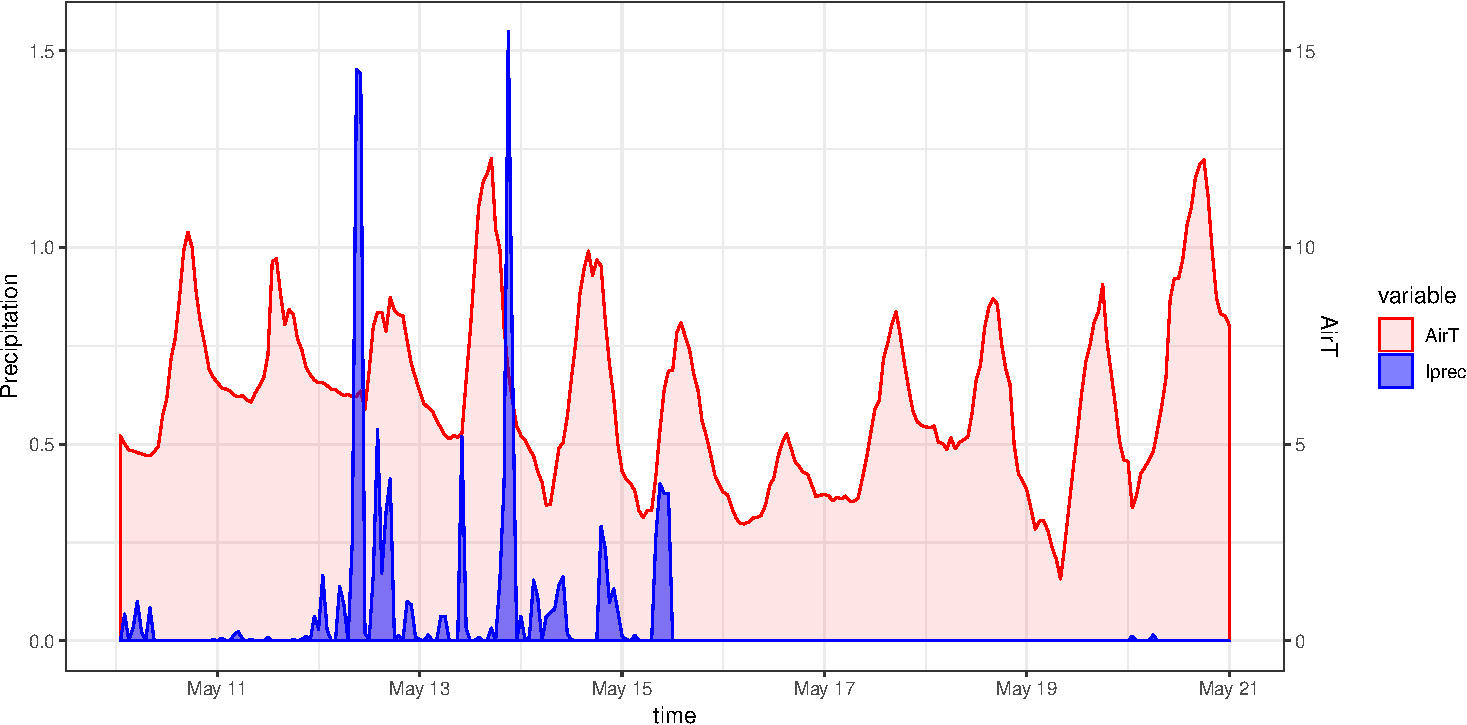
\includegraphics{presentation_files/figure-beamer/unnamed-chunk-6-1.pdf}
\caption{FALSE}
\end{figure}

\end{frame}

\begin{frame}[fragile]{Getting output simulation data at B2}

Soil Water Content Profile:

\begin{Shaded}
\begin{Highlighting}[]
\NormalTok{tz <-}\StringTok{ "Etc/GMT-1"}
\NormalTok{SWC_B2  <-}\StringTok{ }\KeywordTok{get.geotop.inpts.keyword.value}\NormalTok{(}
  \StringTok{"SoilLiqContentProfileFile"}\NormalTok{,}
  \DataTypeTok{wpath =}\NormalTok{ wpath_B2,}
  \DataTypeTok{data.frame =} \OtherTok{TRUE}\NormalTok{,}
  \DataTypeTok{date_field =} \StringTok{"Date12.DDMMYYYYhhmm."}\NormalTok{,}
  \DataTypeTok{tz =}\NormalTok{ tz,}
  \DataTypeTok{zlayer.formatter =} \StringTok{"z%04d"}
\NormalTok{)}
\KeywordTok{help}\NormalTok{(get.geotop.inpts.keyword.value) ## for more details!}
\end{Highlighting}
\end{Shaded}

\end{frame}

\begin{frame}[fragile]{Getting output simulation data at P2}

The same for P2:

\begin{Shaded}
\begin{Highlighting}[]
\NormalTok{wpath_P2 <-}\StringTok{ "resources/simulation/Matsch_P2_Ref_007"} 
\NormalTok{SWC_P2  <-}\StringTok{ }\KeywordTok{get.geotop.inpts.keyword.value}\NormalTok{(}
  \StringTok{"SoilLiqContentProfileFile"}\NormalTok{,}
  \DataTypeTok{wpath =}\NormalTok{ wpath_P2,}
  \DataTypeTok{data.frame =} \OtherTok{TRUE}\NormalTok{,}
  \DataTypeTok{date_field =} \StringTok{"Date12.DDMMYYYYhhmm."}\NormalTok{,}
  \DataTypeTok{tz =} \StringTok{"Etc/GMT-1"}\NormalTok{,}
  \DataTypeTok{zlayer.formatter =} \StringTok{"z%04d"}\NormalTok{)}
\end{Highlighting}
\end{Shaded}

\end{frame}

\begin{frame}{Soil Water Content at P2 and B2}

\begin{figure}
\centering
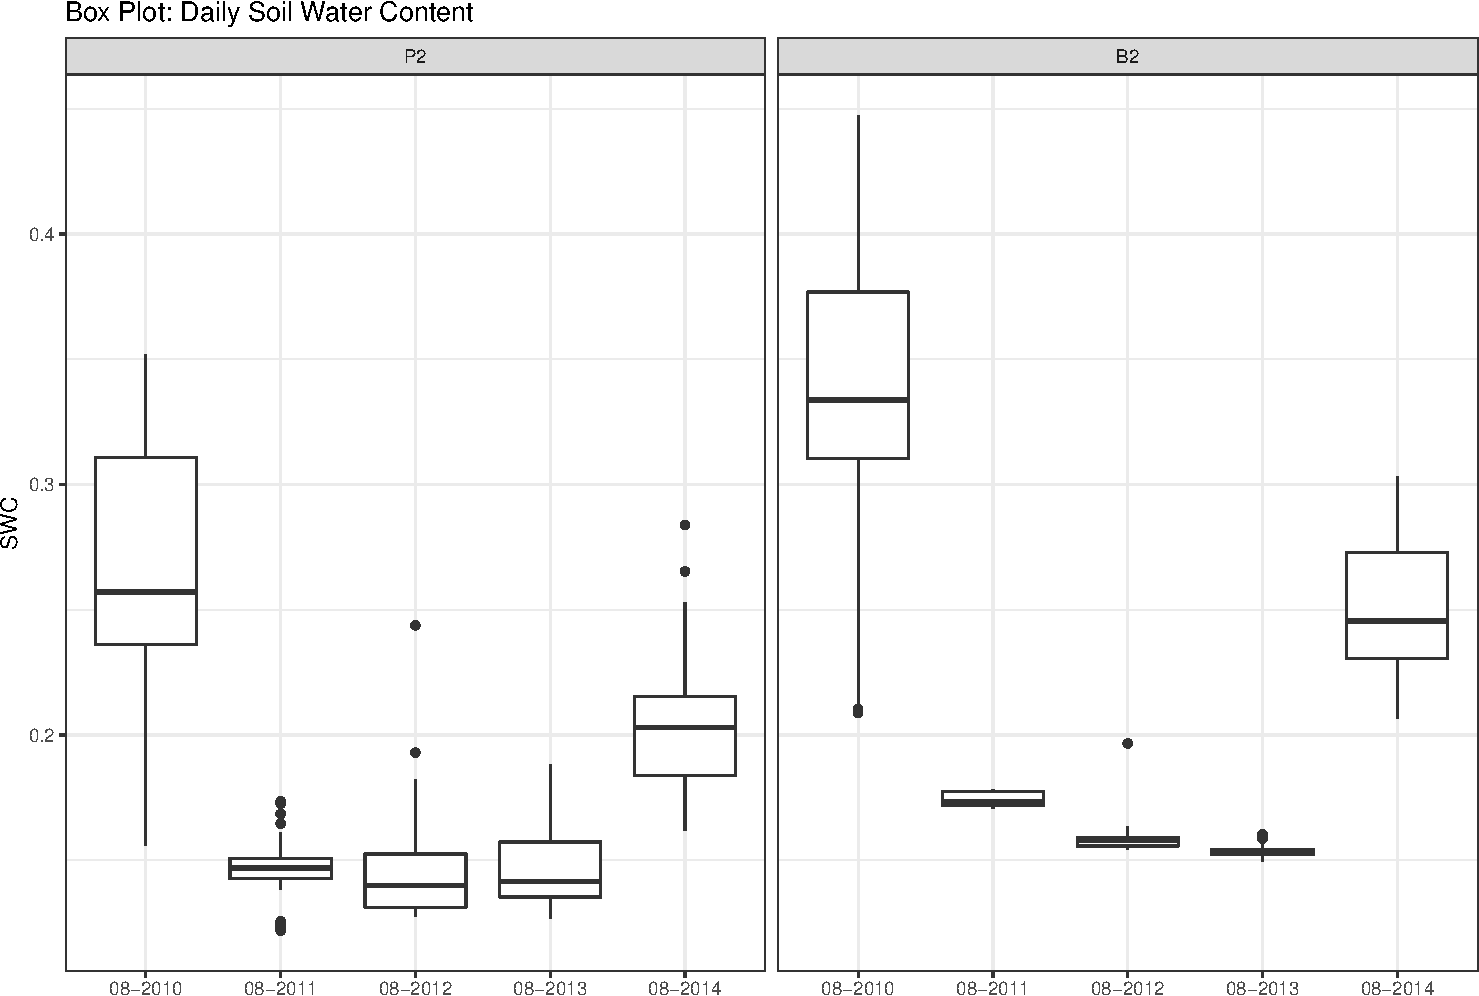
\includegraphics{presentation_files/figure-beamer/unnamed-chunk-11-1.pdf}
\caption{FALSE}
\end{figure}

\end{frame}

\begin{frame}{Output data Analytics (soil Mooisture Distribution)}

Distribution of daily aggregated soil water contant at a 18 cm depth:
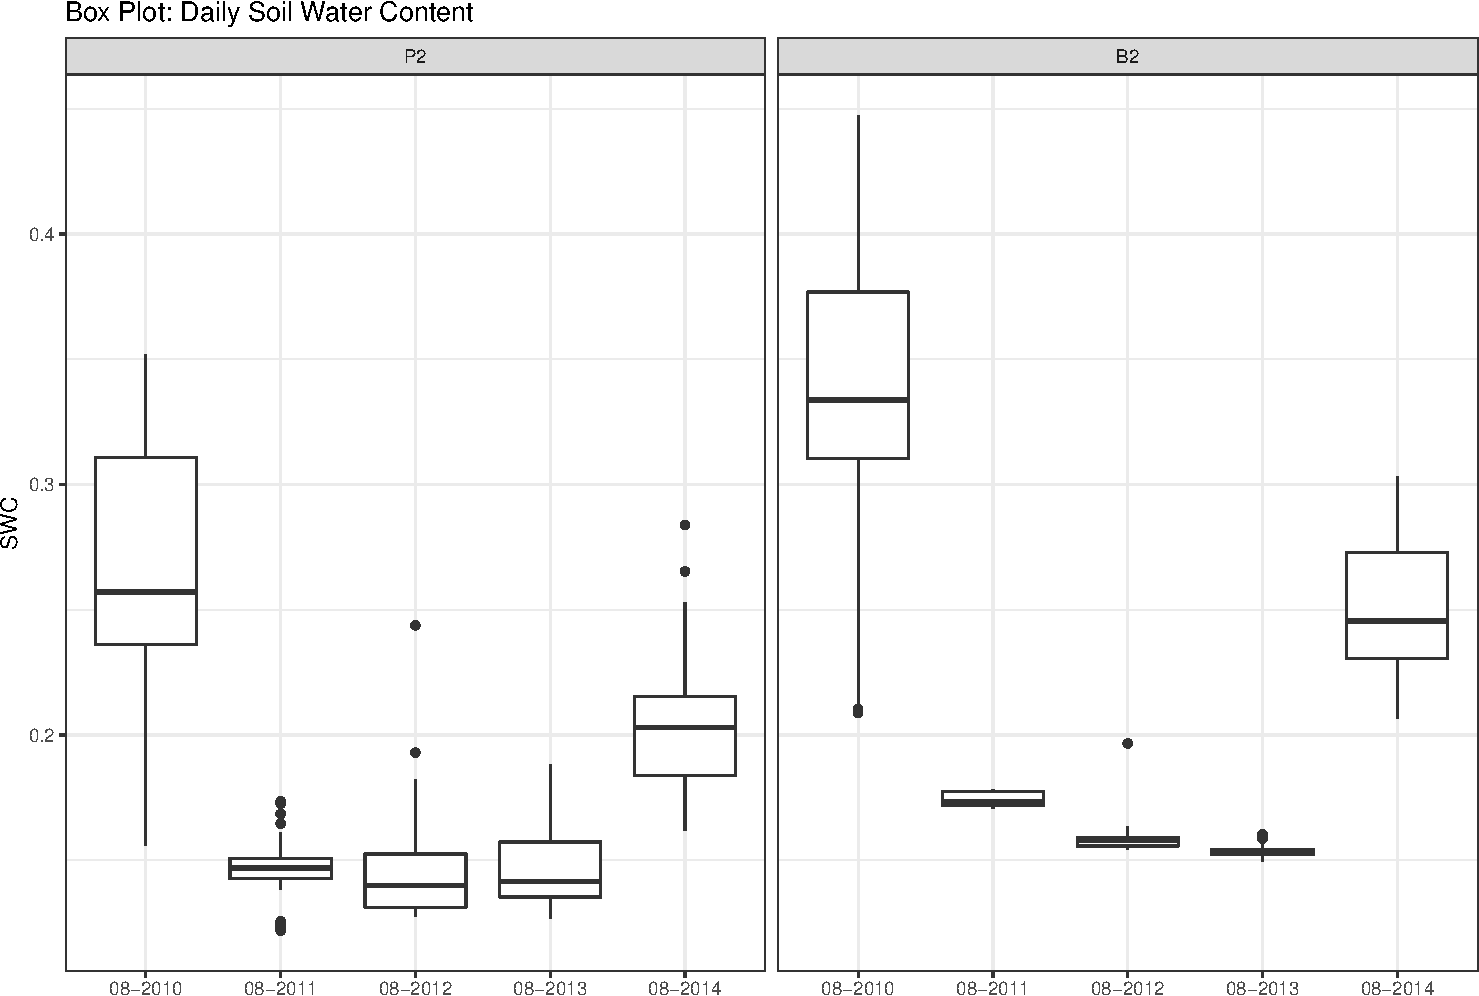
\includegraphics{presentation_files/figure-beamer/unnamed-chunk-12-1.pdf}

More deetails on the
\href{https://github.com/ecor/geotopbricks_doc/blob/master/erum2018_poster/erum2018_poster_cordano_et_al.png}{\textbf{eRum2018}
poster}.

\end{frame}

\begin{frame}[fragile]{3D Spatially Distributed Distribution (Vinschgau
- Upper Adige River Basin - Alps - I/CH/A)}

\begin{Shaded}
\begin{Highlighting}[]
\NormalTok{###wpath_3D <- 'resources/simulation/Vinschgau_test_3D_002'}
\NormalTok{wpath_3D <-}\StringTok{ 'resources/simulation/Mazia'}
\NormalTok{basin <-}\StringTok{ }\KeywordTok{get.geotop.inpts.keyword.value}\NormalTok{(}\StringTok{"LandCoverMapFile"}\NormalTok{,}
              \DataTypeTok{wpath=}\NormalTok{wpath_3D,}\DataTypeTok{raster=}\OtherTok{TRUE}\NormalTok{)}
\NormalTok{basin}
\end{Highlighting}
\end{Shaded}

\begin{verbatim}
## class       : RasterLayer 
## dimensions  : 48, 63, 3024  (nrow, ncol, ncell)
## resolution  : 1000, 1000  (x, y)
## extent      : 598000, 661000, 5145000, 5193000  (xmin, xmax, ymin, ymax)
## coord. ref. : +proj=utm +zone=32 +ellps=WGS84 +datum=WGS84 +units=m +no_defs +towgs84=0,0,0 
## data source : in memory
## names       : layer 
## values      : 1, 11  (min, max)
\end{verbatim}

\end{frame}

\begin{frame}{3D Spatially Distributed Distribution (Input Geospatial
Map)}

\begin{figure}
\centering
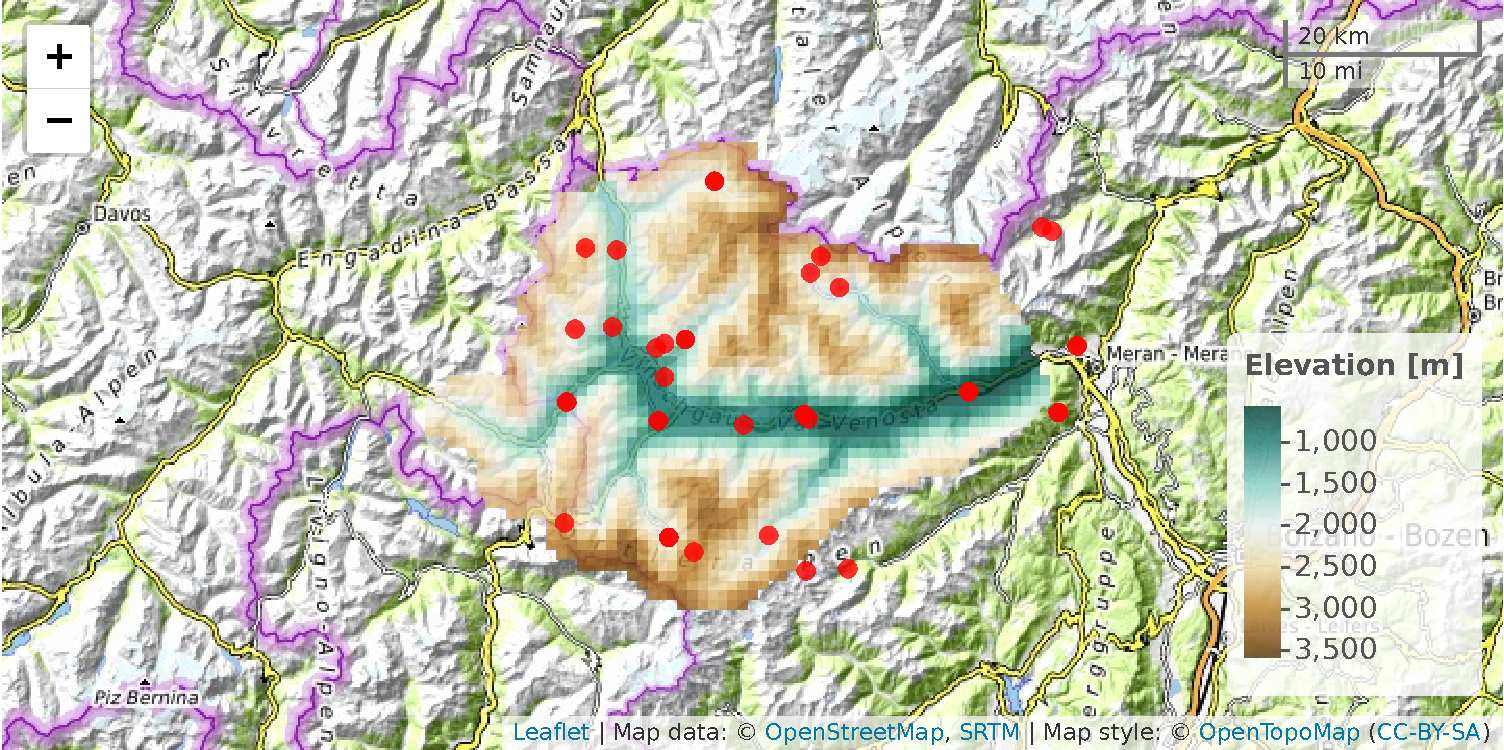
\includegraphics{presentation_files/figure-beamer/unnamed-chunk-14-1.pdf}
\caption{FALSE}
\end{figure}

\end{frame}

\begin{frame}[fragile]{LOREM IPSUM}

\begin{verbatim}
## Warning (get.geotop.inpts.keyword.value): keyword SoilLayerThicknesses without value:
\end{verbatim}

\begin{verbatim}
## [1] "Maps to import: 1 from 2010-10-16 16:00:00 to 2010-10-16 16:00:00"
\end{verbatim}

\begin{verbatim}
## Important bug solved from 1.3.7.3, previous versions (<= 1.3.7.2) could return slightly different results!
\end{verbatim}

\begin{verbatim}
## Importing 2010-10-16 16:00:00
\end{verbatim}

\begin{verbatim}
## As  2010-10-16 16:00:00
\end{verbatim}

\end{frame}

\begin{frame}{3D Simulation Analytics}

The results show than B2 is able to hold more water than P2. This
depends on soil and land properties. Compared with input precipiation
results,soil water behaviour for the different months is related to
precipitation amount (depth and number of rainy days). Interestingly, in
August 2014 soil water content is higher than in August 2012, in which
precipitaion is higher. However, in August 2014 the daily precipitation
distribution is the least wide with the lowest variability
(interquantile range) and two extreme events. (Precipiation time series
in B2 and P2 are equal due to their short distance!)

Hydrological models are solvers of the differantial equations of water
flows and water thermodymanics in the Earth associated to heat transfers
between Earth and the low atmosphere. They are a simplification of a
real-world system useful to understand, predict, manage water resources.
''integrated''

\end{frame}

\begin{frame}{Dicussion}

\begin{itemize}
\tightlist
\item
  open science
\item
  reproducibuly of modelling simulations
\item
  fair priciple
\end{itemize}

\end{frame}

\begin{frame}[fragile]{Conclusion and forward}

\begin{itemize}
\item
  open source hydrolgical models need powerful processing interface
\item
  tool for popsptocesing GEOtop
\item
  getting your data in the right shape (e.g. \texttt{tidyverse},
  \texttt{recipes})
\item
  potential for extension for ohter models
\item
  for oprational aplications / engineering productivity
\item
  enlarge communtiy
\end{itemize}

vedi abstract

\end{frame}

\begin{frame}{Interested?}

www.geotop.org

\begin{itemize}
\tightlist
\item
  link CRAN e github repository
\end{itemize}

Thank you for your attention! / Merci pour votre attention!

\end{frame}

\begin{frame}{Addendum}

LOREM IPSUM

\end{frame}

\end{document}
